\chapter{Results}
\label{chap:results}

\section{Method development}
\label{section:Results_Method_Development}
\subsection{Haemocyte medium: inhibition of aggregation}
The proportions of aggregated haemocytes in \acrshort{mpss}, \acrshort{acb} and \acrshort{mas} are plotted against time post-withdrawal in Figure \ref{fig:aggregation}, together with their predicted mean proportions, or more accurately: the predicted proportion of aggregated haemocytes in mussels with random effects $\gamma_{0i}$ and $\gamma_{1i}$ = 0. Predictions were made from the estimated fixed effects in order to address the marginal effect of "Buffer" on the population-averaged proportions. The estimated regression coefficients of the generalized linear mixed effect model is presented in Table \ref{tb:regression_table}, while the fixed effect sub-models are shown in (\ref{eq:mixed_submodels}).

\begin{equation}
    \label{eq:mixed_submodels}
    y_{ij} = \begin{cases}
        \dfrac{1}{1 + e^{-(-1.7192 + 0.5516 \times log(t_{ij}))}},  & i \: \text{in MPSS group}, \\
        \dfrac{1}{1 + e^{-(-6.9842 + 1.8400 \times log(t_{ij}))}},  & i \: \text{in ACB group}, \\
        \dfrac{1}{1 + e^{-(-7.7198 + 2.0138 \times log(t_{ij}))}},  & i \: \text{in MAS group} \\
    \end{cases}
\end{equation}

Figure \ref{fig:aggregation}D unambiguously demonstrates that both \acrshort{acb} and \acrshort{mas} exerted an immediate decelerating effect on the rate of haemocyte aggregation. This inhibitory effect is evident from the estimated differences in slopes and intercepts from the MPSS sub-model, which were significantly different from zero (see Table \ref{tb:regression_table}). Since the effect sizes are a bit challenging to interpret from the isolated coefficients, the linear predictors of the three sub-models are evaluated on link scale in Figure \ref{fig:LogOdds}, i.e. as predictors for the log odds of the proportion of aggregated haemocytes ($log P(y_{ij} = 1) / P(y_{ij} = 0)$).

\begin{figure}[!ht]
    \centering
    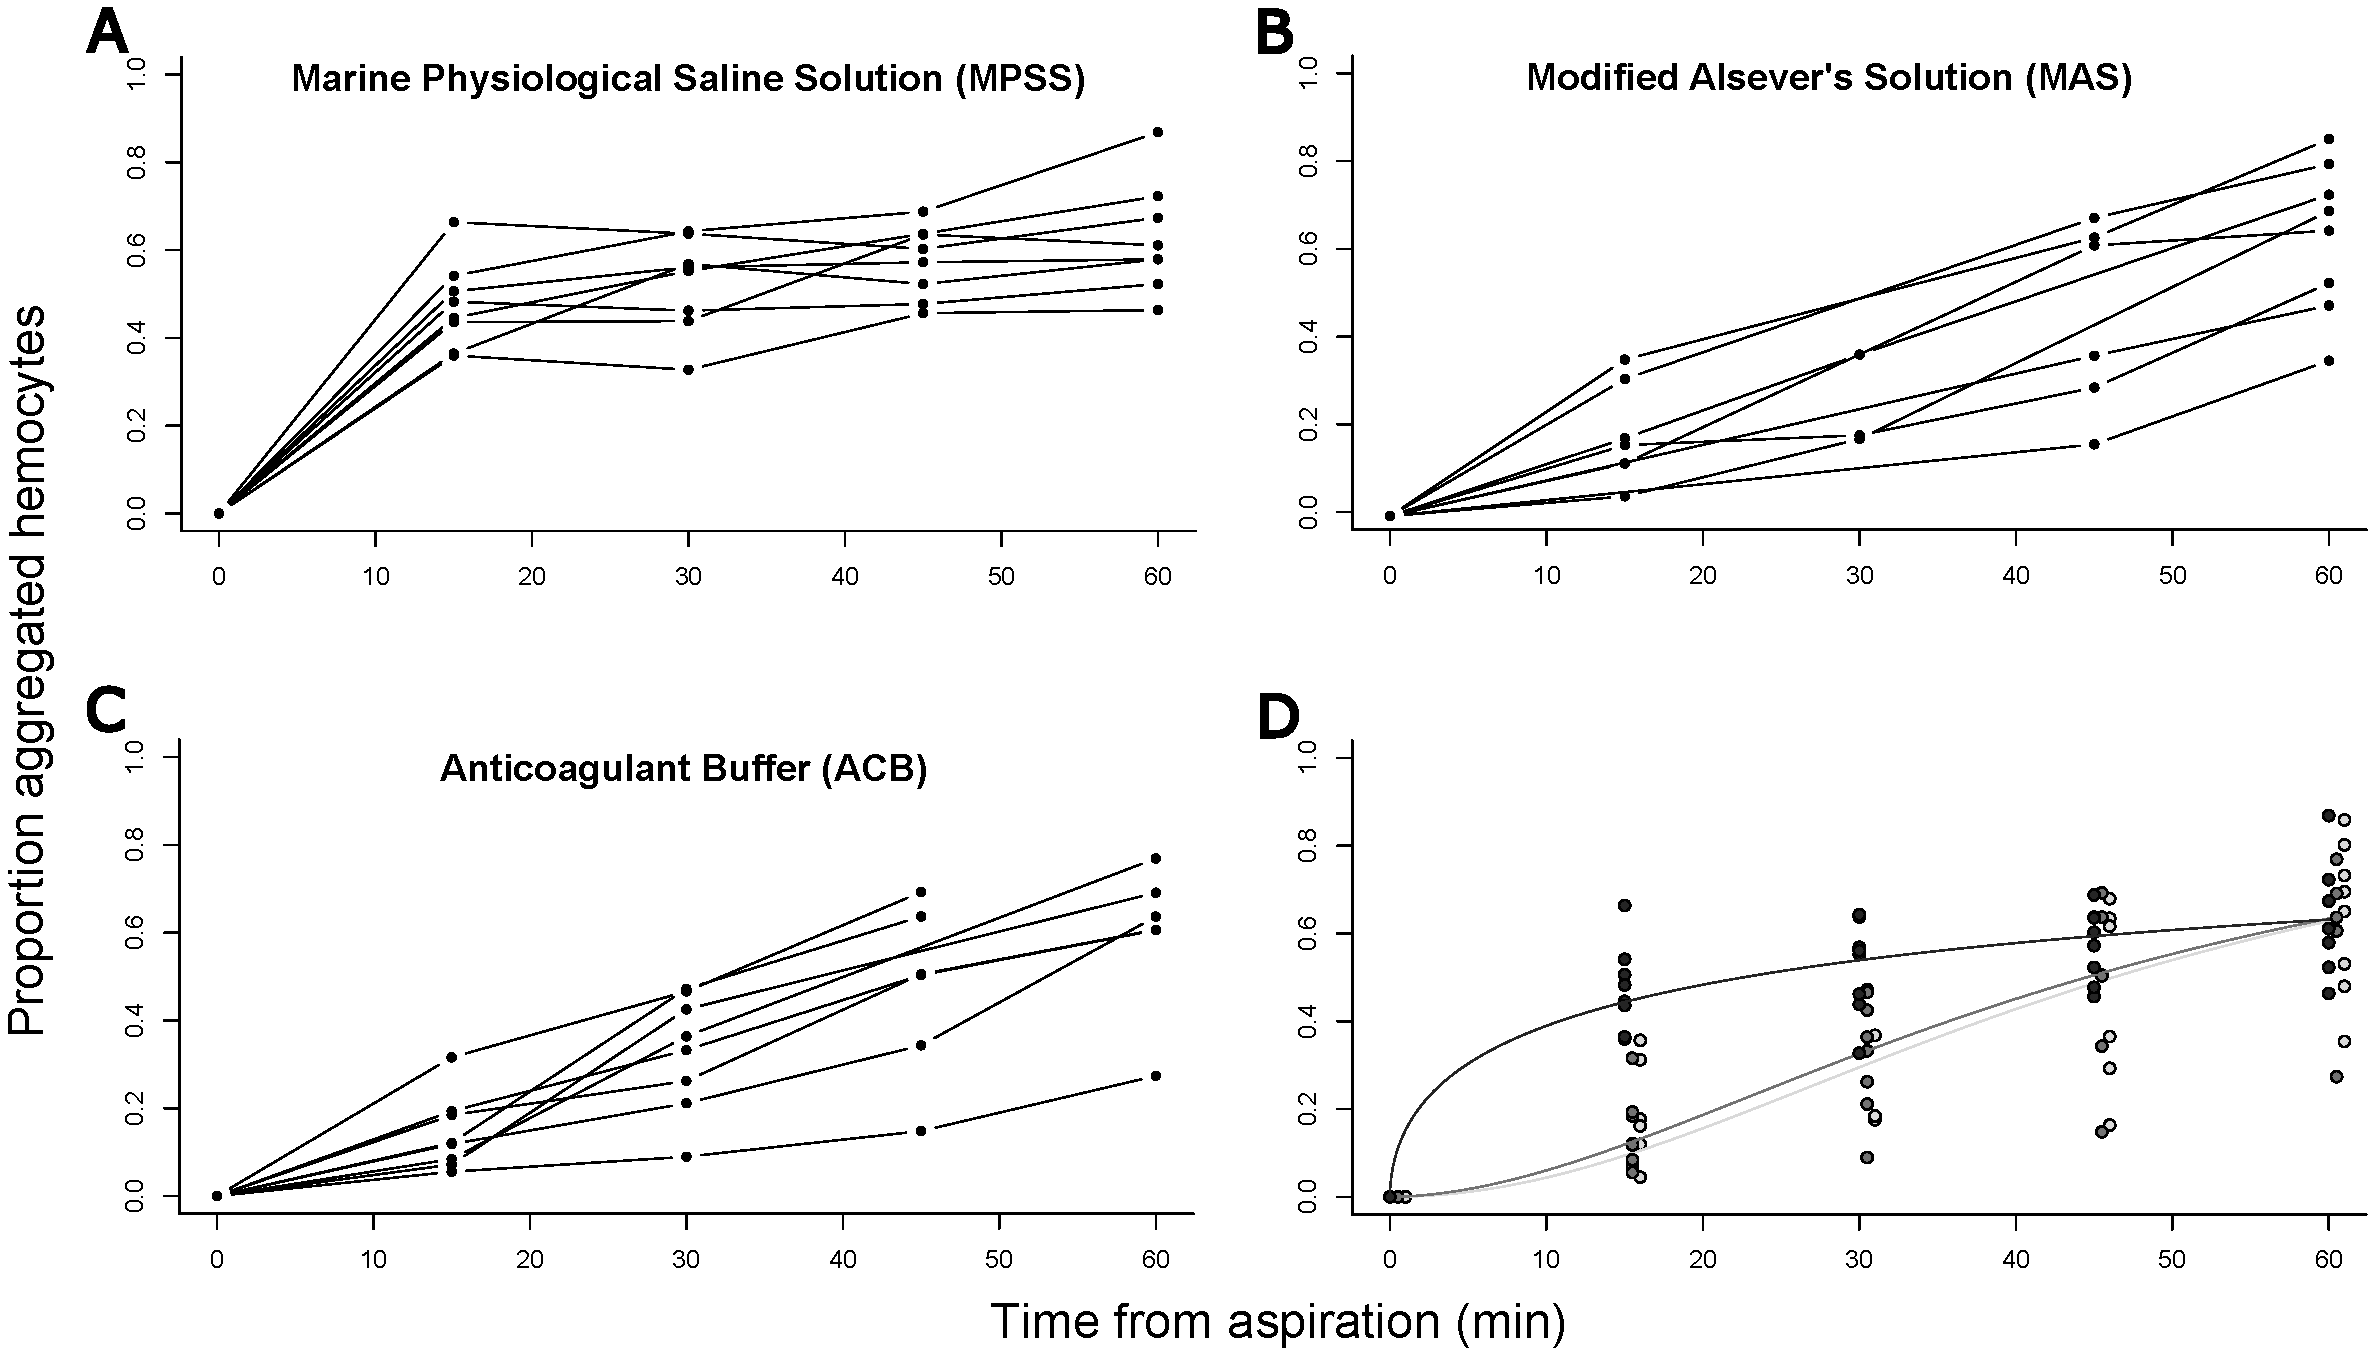
\includegraphics[width=1.0\textwidth]{figures/Method development/Propagg x4 plot.pdf}
    \caption{\textbf{Inhibition of hemocyte aggregation from withdrawing samples into three different anticoagulant buffers.} The proportion of aggregated hemocytes is plotted against time from haemolymph withdrawal after diluting samples in an equal volume of \textbf{A)} Marine Physiological Saline Solution (\acrshort{mpss}, n=8), \textbf{B)} Modified Alsever's Solution (\acrshort{mas}, n=8) or \textbf{C)} Anticoagulant Buffer (\acrshort{acb}, n=8).  \textbf{D)} The same data is combined into one scatter-plot with regression curves representing the mean proportions of aggregated haemocytes in \acrshort{mpss} (\protect\darkgraycircle), \acrshort{mas} (\protect\lysegraacircle) and \acrshort{acb} (\protect\graycircle), as predicted from the fitted mixed logistic regression model. Note that data-points have been jittered on the x-axis to prevent overlap.}
    \label{fig:aggregation}
\end{figure}

\begin{table}[H]
	\centering
	\caption{Parameter estimates of the fitted mixed logistic regression model and their 95\% confidence intervals. Marginal and conditional R$^{2}$-values are presented as parameters of model fit, together with the model's residual deviance.}
	\label{tb:regression_table}
	\begin{tabular}{llllc}
        \toprule
	\textbf{Covariate} & \textbf{Symbol} & \textbf{Estimate$^{b}$} & \textbf{95\% CI$^{a}$} & \textbf{S.E.}\\
		\midrule
  \emph{Intercept}                          & $\alpha_1$ & -1.72*     & [-3.24, -0.202] & 0.740 \\
  \emph{log(t)}                             & $\beta_1$  & 0.552**    & [0.189, 0.915]  & 0.177 \\
  \emph{Buffer$_{ACB}$}                     & $\alpha_2$ & -5.27***   & [-7.41, -3.11]  & 1.05  \\
  \emph{Buffer$_{MAS}$}                     & $\alpha_3$ & -6.00***   & [-8.18, -3.86]  & 1.06  \\
  \emph{log(t)} $\cdot$ \emph{Buffer$_{ACB}$} & $\beta_2$& 1.29***    & [0.775, 1.80]   & 0.251 \\
  \emph{log(t)} $\cdot$ \emph{Buffer$_{MAS}$} & $\beta_3$& 1.46***    & [0.950, 1.98]   & 0.253 \\
  \emph{SD}$(\gamma_{0i})$                  & $\tau_0^2$ & 2.09       & [1.57, 2.91]    & -     \\
  \emph{SD}$(\gamma_{1i})$                  & $\tau_1^2$ & 0.500      & [0.379, 0.694]  & -     \\
  &&& \\
  \multicolumn{5}{l}{Marginal R$^{2}$ = 0.87$^{c}$} \\
  \multicolumn{5}{l}{Conditional R$^{2}$ = 0.98$^{c}$} \\
  \multicolumn{5}{l}{Residual deviance: 13498 on 98 degrees of freedom} \\
		\bottomrule
  \multicolumn{5}{l}{\footnotesize $^{a}$Computed 95\% confidence intervals based on Likelihood Ratio Test of the profile likelihood.} \\
  \multicolumn{5}{l}{\footnotesize $^{b}$ *, **, *** indicates statistical significance on 95\%, 99\% and 99.9\% confidence levels, respectively.} \\
  \multicolumn{5}{l}{\footnotesize Confidence levels were obtained from z-statistics of the asymptotic Wald test.} \\
    \multicolumn{5}{l}{\footnotesize $^{c}$Calculated according to the method proposed by Nakagawa and Schielzeth (2013).} \\
	\end{tabular}
\end{table}

\begin{figure}[!ht]
    \centering
    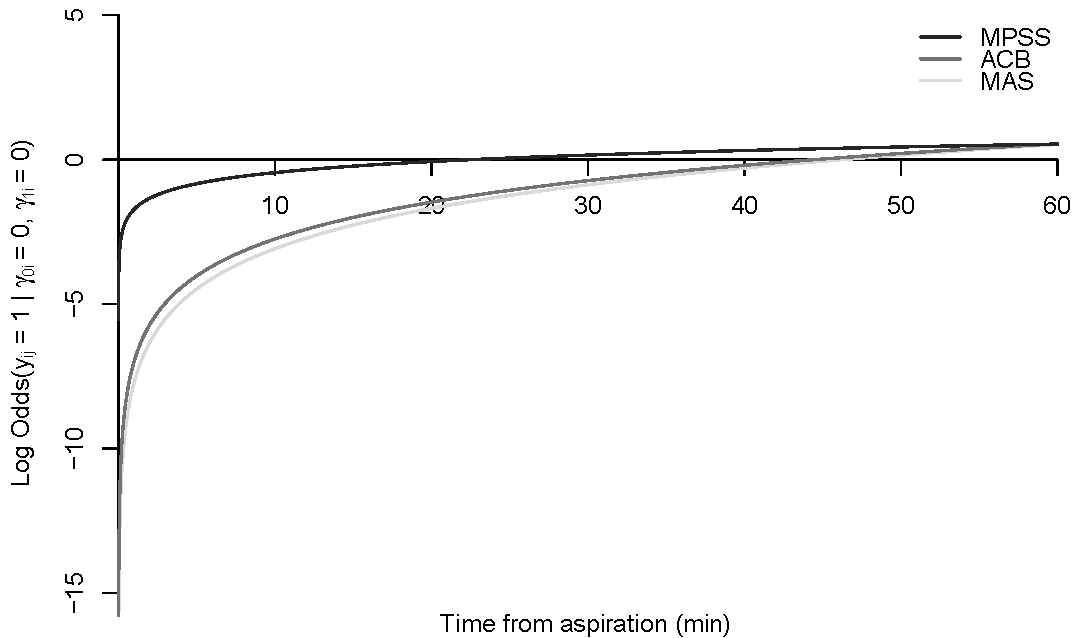
\includegraphics[width=1.0\textwidth]{figures/Method development/Log Odds plot.pdf}
    \caption{The log odds of the proportion of aggregated haemocytes plotted against time (min) after haemolymph withdrawal, when haemolymph samples were withdrawn into Marine Physiological Saline Solution (MPSS), Anticoagulant Buffer (ACB) or Modified Alsever's Solution (MAS). The three curves illustrates the logit-scale predictors of the fitted mixed logistic regression model for the three buffers.}
    \label{fig:LogOdds}
\end{figure}

Given the that the predicted proportion of aggregated haemocytes is 0.50 when the log odds is equal to zero, Figure \ref{fig:LogOdds} shows that 1/2 of the haemocytes withdrawn into \acrshort{mpss} had aggregated within 23 minutes post-withdrawal. This interpretation is valid for mussels where the random effects of time; $\gamma_{0i}$ and $\gamma_{1i}$ = 0. For samples withdrawn into \acrshort{acb} or \acrshort{mas} on the other hand, the cells did not achieve this degree of aggregation until 45 and 46 minutes post-withdrawal, respectively. The three log odds curves depicted in Figure \ref{fig:LogOdds} shows that the inhibitory effects of \acrshort{acb} and \acrshort{mas} were modelled through their significantly lower y-intercepts compared to the \acrshort{mpss} sub-model (Table \ref{tb:regression_table}). Since these estimates were significant after accounting for within-mussel correlations (<.001), we can conclude that \acrshort{edta} is an effective haemocyte anticoagulant on the short term.

The effect was largest during the initial 15-20 minutes, before the degree of aggregation slowly approached that of \acrshort{mpss} around 60 minutes post-withdrawal. In haemolymph samples withdrawn into \acrshort{acb} or \acrshort{mas}, the mean proportions of aggregated haemocytes after 15 minutes were 0.14 95\% CI [0.07, 0.22] and  0.20 95\% CI [0.07, 0.32], respectively. There were no significant differences between the buffers with \acrshort{edta}, but both \acrshort{acb} and \acrshort{mas} had significantly lower proportions at this timepoint compared to samples withdrawn into cold \acrshort{mpss} (0.48 95\% CI [0.39, 0.56]).

Even though the model is over-dispersed, these estimates provide some insight into the three buffers relative abilities to prevent hemocyte aggregation within the first hour post-withdrawal. The combination of a Ca$^{2+}$-free and \acrshort{edta}-containing buffer was effective in reducing hemocyte aggregation compared to simply diluting and keeping samples on ice. When the latter method was used, visible aggregates usually formed within the syringes immediately after hemolymph aspiration, even though the \acrshort{mpss} was pre-chilled on ice. For this method to be effective, the hemolymph most likely has to be diluted many-fold. Such an approach would be inconvenient when preparing haemolymph smears with a certain desired density, and too time-consuming when acquiring 10.000 events on a flow cytometer. This approach was therefore ruled out of question.

Comparing the relative effectiveness of \acrshort{mas} and \acrshort{acb} in preventing hemocyte aggregation, it is evident that neither citrate or maintaining a slightly acidic pH is required for the purpose. It might be that the slightly higher concentration of \acrshort{edta} in \acrshort{acb} compensates for the lack of citrate. But either way, the acidic pH most likely plays a minor role. Since high concentrations of \acrshort{edta} has been reported to impair hemocyte viability (\cite{Grandiosa2018, Burkhard2009}), a direct comparison of \acrshort{mas} and \acrshort{acb} with regards to acute effects on viability was required for a final decision.

\subsection{Haemocyte medium: effect on viability}
 The mean percentages of necrotic hemocytes in \acrshort{mpss}, \acrshort{acb} and \acrshort{mas} after 15 minutes, 2 hours and 20 hours incubation are presented in Figure \ref{fig:BufferViability}, with error bars representing 95\% confidence intervals around group means. Within group differences in means at the three incubation periods are presented Table \ref{tb:Paired_ttests}.

\begin{figure}[!ht]
    \centering
    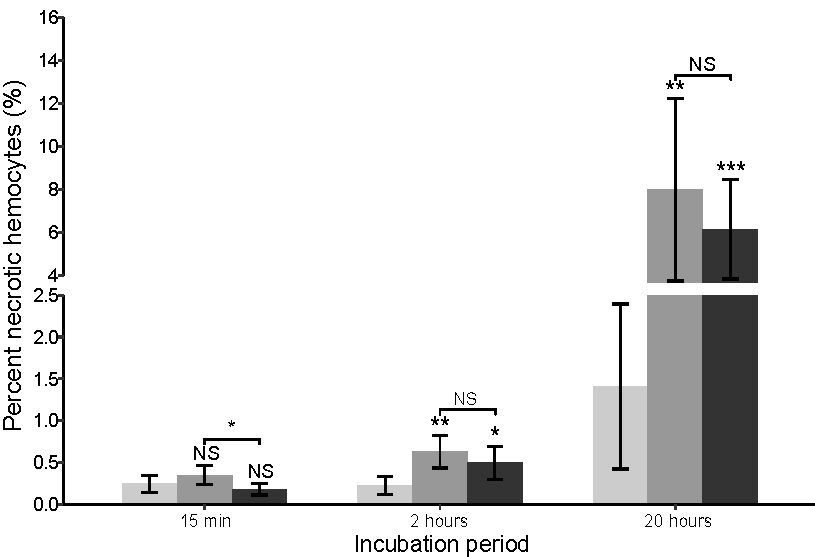
\includegraphics[width=0.75\textwidth]{figures/Method development/buffer viability bargraph scaled.pdf}
    \caption{The mean percentages of TO-PRO$^{TM}$-3 Iodide positive hemocytes after 15 minute, 2 hours and 20 hours incubation in Marine Physiological Saline Solution (\, \protect\lysegraabox, \ n=8), Anticoagulant Buffer (\, \protect\customgraybox, \ n=8) and Modified Alsever's Solution (\, \protect\darkgraybox, \ n=8). Error bars represent 95\% confidence intervals around group means, asterisks *, **, *** above error bars denotes confidence level of one-tailed two sample t-test comparisons with the \acrshort{mpss} control group, while asterisks above horizontal lines represent \acrshort{acb} vs. \acrshort{mas} comparisons.}
    \label{fig:BufferViability}
\end{figure}

The difference between the negative control group (\acrshort{mpss}) and the two \acrshort{edta}-containing buffers were not significantly different from zero after 15 minute incubation. There was however a marginal difference between \acrshort{mas} and \acrshort{acb}, where samples incubated in \acrshort{acb} had 0.17\% more necrotic cells on average compared to those kept in \acrshort{mas} for 15 minutes (t(14) = 2.96, p=.005). This relationship was consistent across all three incubation periods, allthough the differences after 2 and 20 hours were not significantly different from zero (Figure \ref{fig:BufferViability}).

Moreover, as the incubation period was increased to 2 and 20 hours, the percentages of necrotic haemocytes in \acrshort{acb} and \acrshort{mas} increased relative to the negative control group. After 2 hours incubation, there were 0.40\% and 0.27\% more necrotic haemocytes in \acrshort{acb} (t(14) = 4.29, p<.001) and \acrshort{mas} (t(14) = 2.86, p=.006) compared to cold \acrshort{mpss}, respectively. After 20 hours incubation, these differences had increased to 6.96\% (t(14) = 3.78, p=.003) and 5.12\% (t(14) = 4.82, p<.001).

\begin{table}[h]
\centering
	\caption{Paired two-tailed t-tests were used to assess wether the percentages of necrotic haemocytes increased with incubation time within each group. The difference between means at t = 15 min, 2 hours and 20 hours are presented with 95\% confidence intervals and the belonging p-value.}
	\label{tb:Paired_ttests}
        \resizebox{\linewidth}{!}{
	\begin{tabular}{c|ccccc}
		\toprule
		\multirow{2}{*}{Buffer} & \multicolumn{2}{c}{\textbf{Paired t-test comparison}} & \multirow{2}{*}{Difference (\%)} & \multirow{2}{*}{95\% CI} & \multirow{2}{*}{Pr(T > $\mid$ t $\mid)$} \\
		& Incubation \emph{t} & Incubation \emph{t - 1} & & & \\
		\midrule
     \multirow{2}{*}{MPSS} &  2 hours  &  15 min  & -0.018 & [-0.023, -0.015] & .78 \\
     &  20 hours &  2 hours & 1.184  & [1.157, 1.211]   & .026 \\
    &&&&& \\
    \multirow{2}{*}{ACB} &   2 hours  &  15 min  & 0.279  & [0.272, 0.285]   & .025 \\
       &   20 hours &  2 hours & 7.742  & [7.627, 7.857]   & .00324 \\
    &&&&& \\
    \multirow{2}{*}{MAS} &   2 hours  &  15 min  & 0.319  & [0.313, 0.324]   & .00690 \\
        &   20 hours &  2 hours & 6.037  & [5.970, 6.105]   & <.001 \\
		\bottomrule
	\end{tabular}
 }
\end{table}

These results would suggest that \acrshort{edta} is cytotoxic to haemocytes at the concentrations used in \acrshort{acb} (13.4 mM) and \acrshort{mas} (11.5 mM), since there was a significant dose-dependent increase in the percentage of necrotic haemocytes when \acrshort{acb} and \acrshort{mas} were used as anticoagulants (Table \ref{tb:Paired_ttests}). However, since there was no significant differences between the \acrshort{edta}-containing buffers and the negative control group after 15 minutes of incubation, this cytotoxic effect has no relevant manifestations within the time-frame of the planned flow cytometric analyses. As long as haemolymph samples are stained and processed within 30 minutes of sampling, a flow cytometric dye exclusion/inclusion assay with TO-PRO$^{TM}$-3 Iodide and \acrshort{calceinam} should not have time to detect \emph{in vitro} necrosis caused by the buffers themselves.

\subsection{Cytologic characterization of \emph{M. edulis} hemocyte subpopulations}
\label{subsection:Results_cytchar}
The hemolymph of \emph{Mytilus edulis} comprised a mixed population of cells differing in size, granularity, morphometrics and Wright's-Giemsa staining profiles. If the haemocytes were allowed to spread prior to fixation and staining, the diversity further expanded as cells took on a variety of shapes and/or developed cytoplasmic extensions. From these morphological criteria, a total of three distinct cell types could be identified by light microscopy.

\begin{figure}[H]
    \centering
    \includegraphics[width=1.0\textwidth]{figures/Anatomy/cell types brightfield updated 2.pdf}
    \caption{100$\times$ brightfield micrographs of the three haemocyte types found in the haemolymph of \emph{Mytilus edulis}, fixed and stained on glass slides with the Hemacolor\textsuperscript{\textregistered} kit before the hemocytes had time to spread notably. \textbf{(A-E)} Blast-like hyaline basophils. \textbf{(F-J)} Basophilic granulocytes. \textbf{(K-O)} Eosinophilic granulocytes. Samples were withdrawn into \acrshort{mpss} (1:1), scale bars = 10 \micro m.}
    \label{fig:celltypes}
\end{figure}

Based on the basophilic or eosinophilic nature of their granules and other cytoplasmic contents, cytologic staining with 3 \% Wright's-Giemsa or the Hemacolor\textsuperscript{\textregistered} kit gave rise to two distinct staining profiles: basophilic and eosinophilic haemocytes. The cytoplasm of eosinophilic hemocytes (Figure \ref{fig:celltypes}, K-O) were densely packed with pink to dark purple granules of varying size and abundance. Hence, they are referred to as eosinophilic granulocytes herein. Their individual granules were usually not distinguishable in a non-spread state, but instead gave their cytoplasm an irregular pink color (Figure \ref{fig:celltypes}, K and O). These haemocytes had cell diameters in the range of 6-16 \micro m, with a mean of 9.06$\pm1.25$ \micro m. Two strikingly homogeneous features of this cell type was a small acentrically located nucleus, and a regular spherical outline in a non-spread state. With abundant pink cytoplasm making up the majority of the cells' surface area - even in the smallest specimens - the eosinophilic granulocytes could also be characterized by a low nuclear-cytoplasmic ratio (N:C ratio). If not fixed and stained before smearing - or within minutes of applying haemolymph to a glass slide - eosinophilic granulocytes were almost exclusively observed as spread cells. 

Compared to the eosinophilic granulocytes, the basophilic hemocytes encompassed a more heterogeneous population. Common to all of them were a larger nucleus that occupied more of the cells' total surface area (higher N:C ratio). The shape of which varied from spherical to oval, or had a distinct bean-shaped or irregular outline. But judged from the morphological criteria of cell size, granularity and N:C ratio, there were essentially two distinct subpopulations of basophilic haemocytes: one population of small hyaline blast-like haemocytes (5.63 $\pm{0.72}$ \micro m) displaying only a marginal rim of dove blue cytoplasm and no apparent cytoplasmic granules (Figure \ref{fig:celltypes}, A-E), and one population of larger haemocytes (8.07 $\pm{1.25}$ \micro m), displaying abundant basophilic cytoplasm with varying degrees of cytoplasmic granulation and vacuolation (Figure \ref{fig:celltypes}, F-J). The basophillic granules appeared much smaller than those of the eosinophilic granulocytes, and were usually not very conspicuous unless haemocytes were subjected to osmotic swelling prior to fixation and staining. Under differential interference contrast (DIC) illumination however, their granules created highly irregular surface topographies in spread cells that could be observed without such treatment. On the basis of these morphological differences, the basophilic haemocytes were subdivided into blast-like haemocytes and basophilic granulocytes herein. 

\begin{figure}[H]
    \centering
    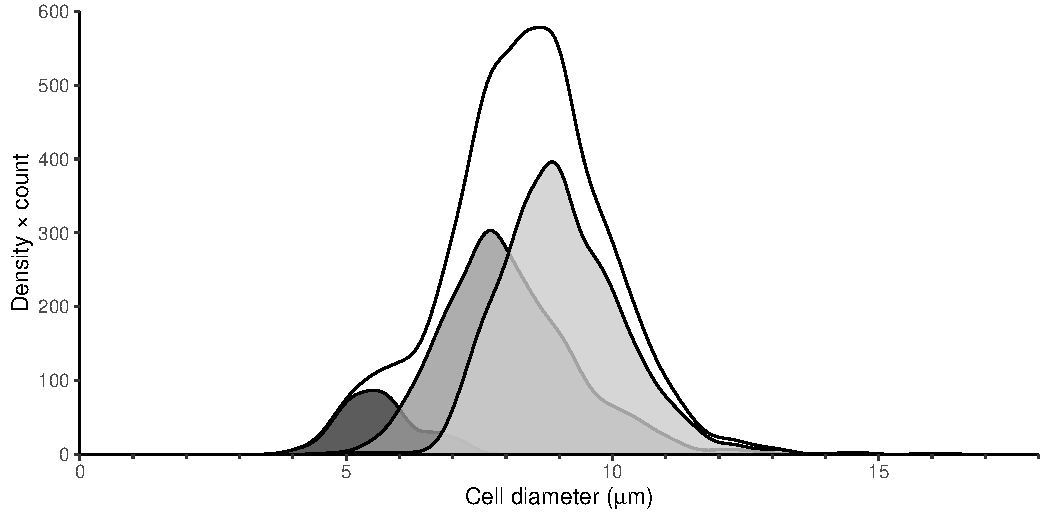
\includegraphics[width=1.0\textwidth]{figures/Anatomy/diameters scaled density plot.pdf}
    \caption{Size distribution of \protect\dimgraybox \ small blast-like basophils (n=154), \protect\lightgraybox \ basophilic granulocytes (n=821), \protect\lysegraabox \ eosinophilic granulocytes (n=1030) and \protect\whitebox \ the total haemocyte population of \emph{Mytilus edulis} (n=2005). The diameters of 100 formaldehyde-fixed haemocytes were measured in each of 20 individual mussels, and the density was scaled to the number of observations of each cell type.}
    \label{fig:Diameters}
\end{figure}

The size distributions of the three haemocyte types are shown as three kernel-smoothened density plots in Figure \ref{fig:Diameters}, together with that of the total haemocyte population. The densities have been scaled to the number of observations of each cell type, such that their relative proportions can be visualized. In the 20 adult mussels examined here, the small blast-like basophils were the least abundant cell type, making up 7.9 $\pm{5.6}$\% of the total haemocyte population. In 14 out of 20 mussels, the blast-like basophils were followed by the basophilic granulocytes, with a mean relative proportion of 40.7 $\pm{12.9}$\%. In spite of constituting similar proportions as the basophilic granulocytes in several mussels, the eosinophilic granulocytes were the most abundant cell type in the haemolymph of \emph{M. edulis}, constituting 51.5 $\pm{15.3}$\% of the total haemocyte population, on average. The relative proportions of basophilic and eosinophilic granulocytes did however vary to a large extent between individual mussels, as reflected by their standard deviations. [Should I include t.tests in this section? - note: unequal sample sizes]

When incorporating the Coulter Counter data in this section, this article can be used to reference the accuracy of the electronic cell size method which it uses: Mattern CFT, Brackett FS, Olson BJ. Determination of number and size of particles by electrical gating: blood cells. J Appl Physiol 1957;10:56–70


\subsection{Flow cytometric characterization of haemocyte subpopulations by light-scatter}
\label{subsection:Results_FlowChar}
A maximum of three distinct subpopulations could be separated according to Forwards scatter (FCS) vs. Side scatter (\acrshort{ssc}) in suspensions of living haemocytes. These comprised one subpopulation of events with low \acrshort{fsc}- and \acrshort{ssc}-values, one subpopulation with high \acrshort{fsc} and intermediate \acrshort{ssc}-values and one subpopulation with high \acrshort{fsc} and \acrshort{ssc}. The aforementioned subpopulations correspond to clusters 1, 2 and 3 in Figure \ref{fig:fsc_vs_ssc}, where the haemocytes of three representative mussels have been displayed with \acrshort{ssc} on logarithmic and linear scales.

The adjunct histograms in Figure \ref{fig:fsc_vs_ssc}A and B clearly illustrates that the three clusters of events are separated according to log \acrshort{ssc}, while there is substantial overlap between cluster 2 and 3 with regard to \acrshort{fsc}. The latter feature was consistent across all mussels, while the degree of separation according to log \acrshort{ssc} was subject to individual variation. In this regard, the haemolymph sample presented in \ref{fig:fsc_vs_ssc}B represents a typical mussel, i.e., with cluster 2 and 3 incompletely separated according to log \acrshort{ssc}. The samples presented in \ref{fig:fsc_vs_ssc}A and C represents the extreme ends of this variation, with complete separation and complete overlap, respectively.

Since \acrshort{fsc} and \acrshort{ssc} can be interpreted as relative measures of cell size and internal complexity, these results suggests that the haemolymph of \emph{M. edulis} are comprised of three cell types that are distinguishable according to size and internal complexity. The events populating cluster 1 exhibited low \acrshort{fsc}- and \acrshort{ssc}-values relative to cluster 2 and 3, indicating that it is populated by haemocytes that are both smaller and less complex than the rest of the haemocytes. If \acrshort{ssc} is interpreted more specifically in terms of haemocyte characteristics, the events populating cluster 2 and 3 most likely correspond to large semi-granular haemocytes and large granulocytes, respectively.

\begin{figure}[!ht]
    \centering
    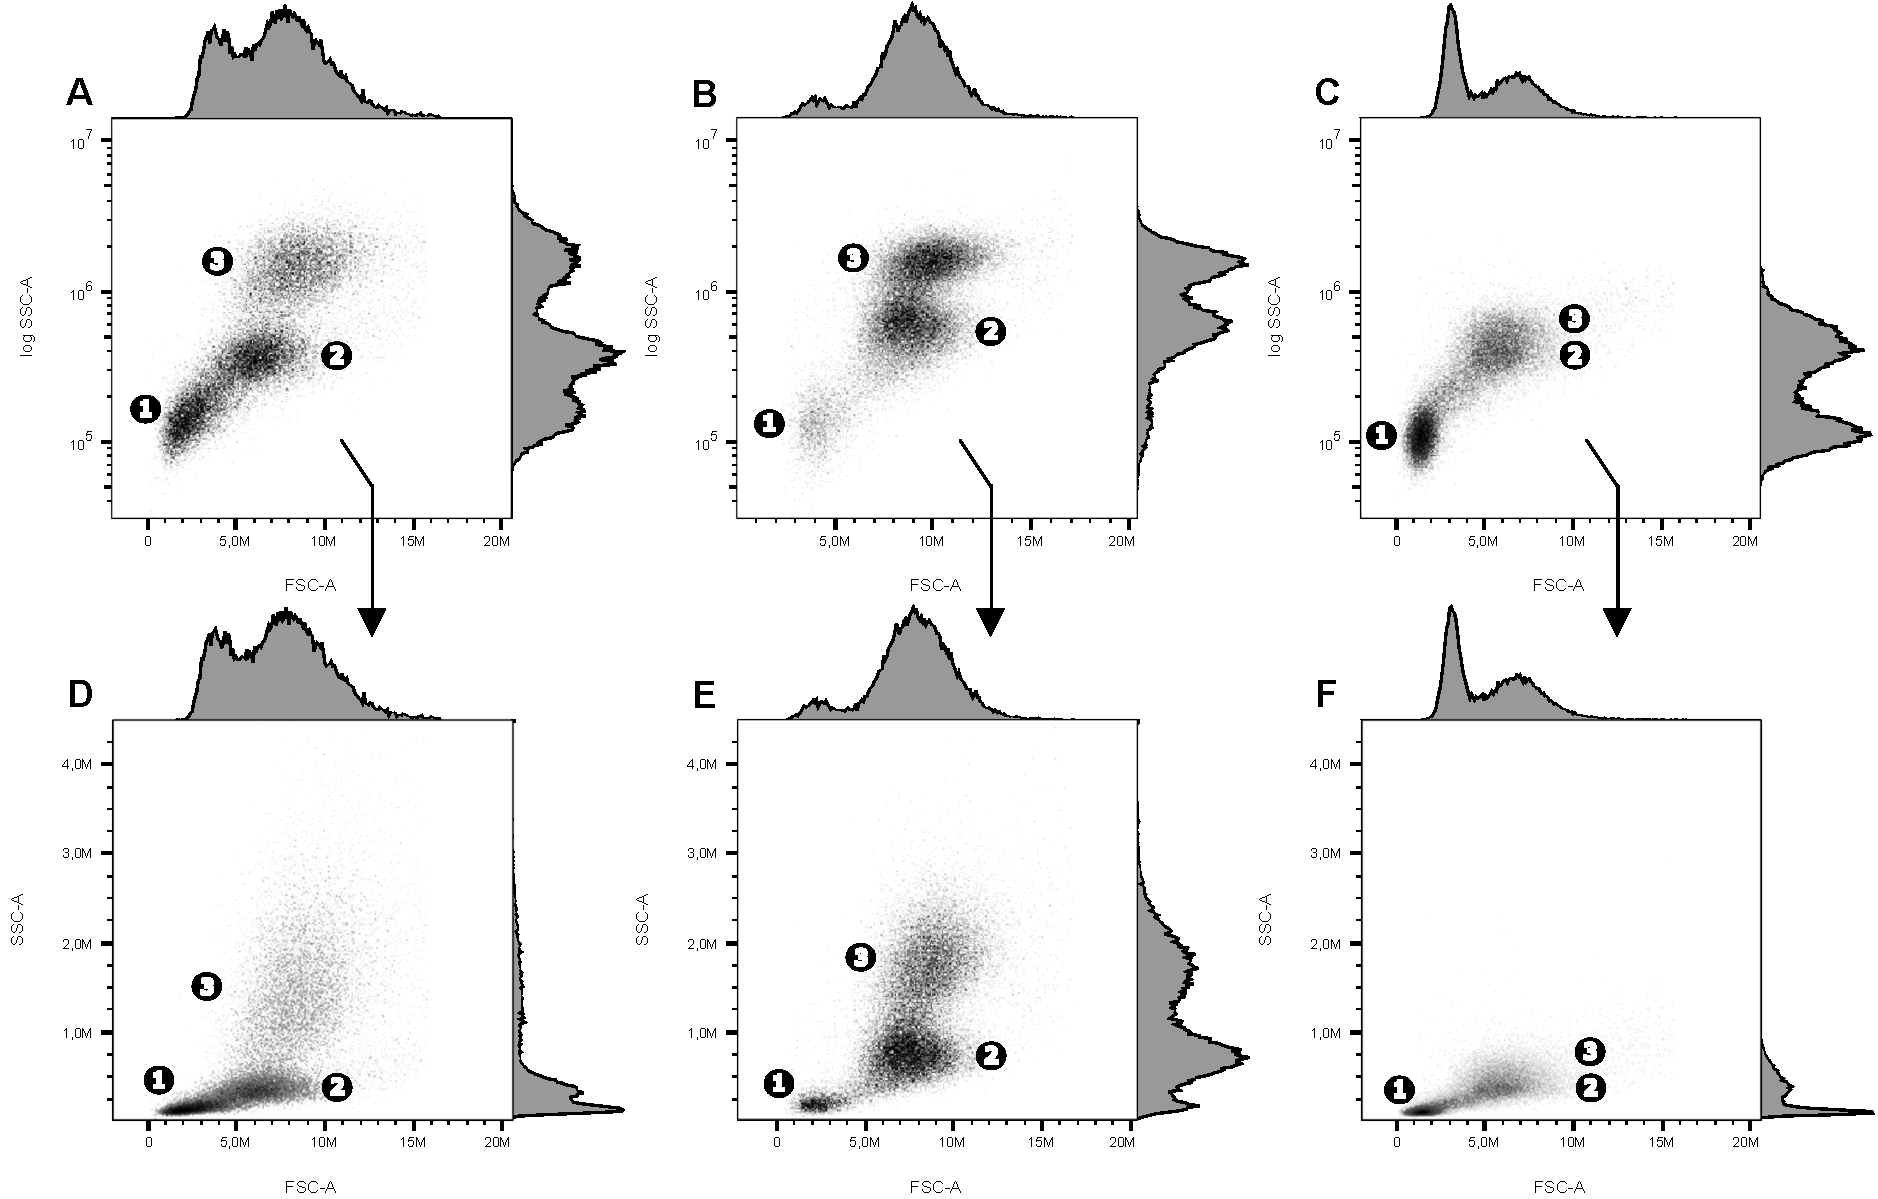
\includegraphics[width=1.0\textwidth]{figures/Gating strategy/30k scatter profiles musc.pdf}
    \caption{\textbf{Haemocyte subpopulations distinguishable according to \acrshort{fsc} and \acrshort{ssc} measurements with the BD Accuri C6 Plus Benchtop Flow Cytometer.} The light-scatter profiles of three representative adult mussels are displayed with \acrshort{ssc} on logarithmic \textbf{(A-C)} and linear \textbf{(D-F)} scales to illustrate the observed variation in the degree of separation between cluster 2 and 3. Adjunct histograms were included to underline the degree of separation from the individual parameters.}
    \label{fig:fsc_vs_ssc}
\end{figure}

When these results are viewed in light of the three cytologically defines cell types of section \ref{subsection:Results_cytchar}, it is not hard to deduce which cell types these three clusters are expected to represent. The small blast-like basophilic haemocytes (5.63 $\pm{0.72}$ \micro m) were considerably smaller than the basophilic and eosinophilic granulocytes, and exhibited no apparent granulation. In other words, they were expected to be unambiguously separated from the larger granulocytes according to both \acrshort{fsc} and \acrshort{ssc}. There might be a slight overlap in size between the largest blast-like haemocytes and the smallest basophillic granulocytes in some mussels (see Figure \ref{fig:Diameters}), however; since they are uncomplex cells, they should be separated according to \acrshort{ssc} regardless. The events populating cluster 1 in Figure \ref{fig:fsc_vs_ssc} are therefore expected to represent small blast-like basophilic haemocytes. 

Both eosinophilic and basophilic granulocytes were granulated in the formal definition of the word. But this discussion requires a more nuanced interpretation of what is meant by granulocyte herein. The cytoplasm of eosinophilic granulocytes were packed with pink to dark purple granules to the extent that their cytoplasm appeared pink in a non-spread state. This stands in sharp contrast to the granulation of basophilic granulocytes, which were more sparse, variable and much less conspicuous. Consequently, there is little doubt that cluster 3 is expected to correspond to eosinophilic granulocytes, while the semi-granular events of cluster 2 aligns with the size and complexity of basophilic granulocytes.

As seen from the size distributions in Figure \ref{fig:Diameters}, the basophilic and eosinophilic granulocytes were not readily distinguishable according to cell size. That result was further substantiated by the fact that cluster 2 and 3 have substantially overlapping \acrshort{fsc}-values. The haemolymph samples depicted in Figure \ref{fig:fsc_vs_ssc} does however show that the \acrshort{fsc} of cluster 3 is slightly right-shifted relative to cluster 2, which is expected since the eosinophilic granulocytes were found to be 0.92 \micro M larger than basophilic granulocytes on average (t(1994) = 18.95, p<.001).

Even thought there is an apparent correlation between cluster 1-3 and the size and internal complexity of the cytologically defined cell types; these interpretations require visual verification before a potential gating strategy can be implemented from these results.

\subsection{Relating the cytologically defined cell types to light-scatter profiles}


The first round of Percoll separation yielded 96.1 \% eosinophilic granulocytes in the 43/90\% fraction.
The second round of percoll gradient separation yielded: 15\%-33\% interface: FCM = 97\% basophils, microscopy = 96.14 \% basophils (7.72\% blast-like and 88.42\%) (= 3.86 \% eosinophils) 43\%-90\% interface: FCM = 94\%, microscopy = 97.52 \%.

\begin{figure}[!ht]
    \centering
    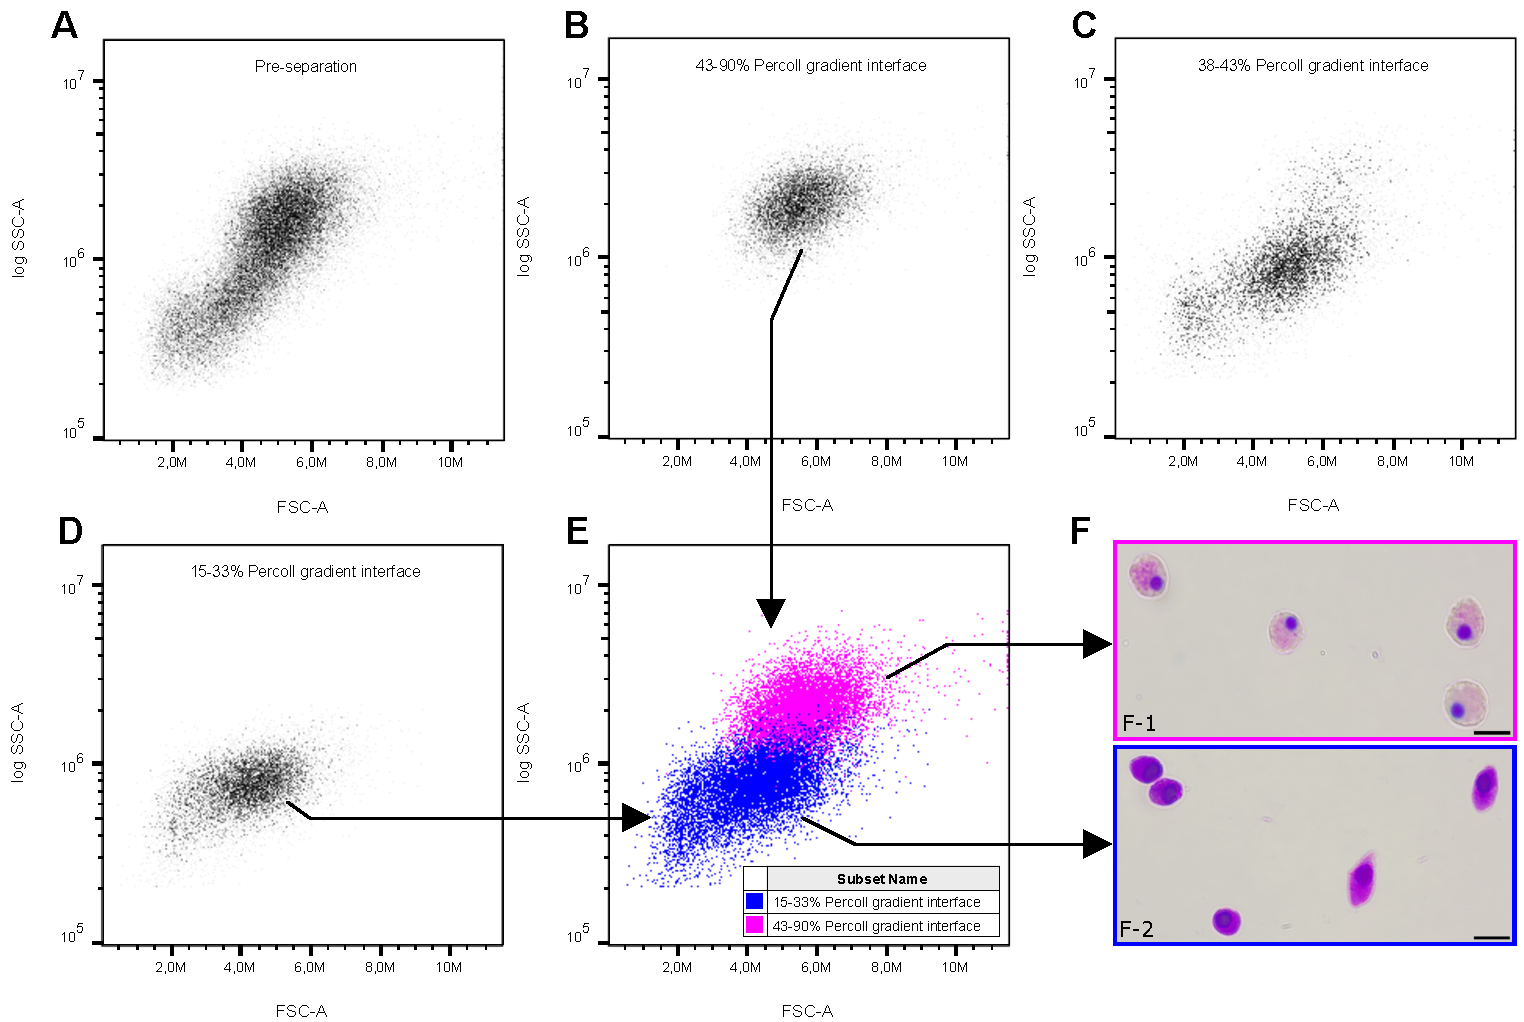
\includegraphics[width=1.0\textwidth]{figures/Method development/PERCOLL SEP II.pdf}
    \caption{\textbf{Confirmation of the light scattering profiles of eosinophilic and basophilic granulocytes pre-separated by discontinuous density centrifugation. A} Light scattering profile of the 95\% pure eosinophilic fraction that separated out on top of the 43-90\% Percoll gradient interface. \textbf{B} Bla bla bla eosin separation bla bla...}
    \label{fig:Percoll-dotplots}
\end{figure}

\begin{figure}[H]
    \centering
    \begin{subfigure}[b]{.45\textwidth}
        \centering
        \includegraphics[width=\textwidth]{figures/Method development/B2A eosin fluorescence/Epi eosin fluorescence.pdf}
        \caption{Hemocytes imaged under brightfield illumination.}
        \label{ffig:a}
    \end{subfigure}
    \hfill
    \begin{subfigure}[b]{.45\textwidth}
        \centering
        \includegraphics[width=\textwidth]{figures/Method development/B2A eosin fluorescence/Brightfield eosin fluorescence.pdf}
        \caption{Haemocytes imaged by epifluorescence microscopy with a B-2A filtercube.}
        \label{ffig:b}
    \end{subfigure}
    \caption{\textbf{Eosinophilic granulocytes are distinguished from the two basophilic cell types according to eosin fluorescence ($\geq$ 515 nm).} Formaldehyde-fixed haemocytes stained in 0.75\% eosin and 3\% Giemsa were imaged at $\times$60 under \textbf{a)} brightfield illumination and \textbf{b)} by epifluorescence microscopy with a B-2A filter cube. The slide was mounted with Eukitt\textsuperscript{\textregistered} and coverslipped prior to microscopy. Eo: eosinophilic granulocyte; B: basophilic haemocyte; scale bars = 10 \micro m. }
    \label{fig:Eosin_fluorescence_B2A}
\end{figure}


\begin{figure}[!ht]
    \centering
    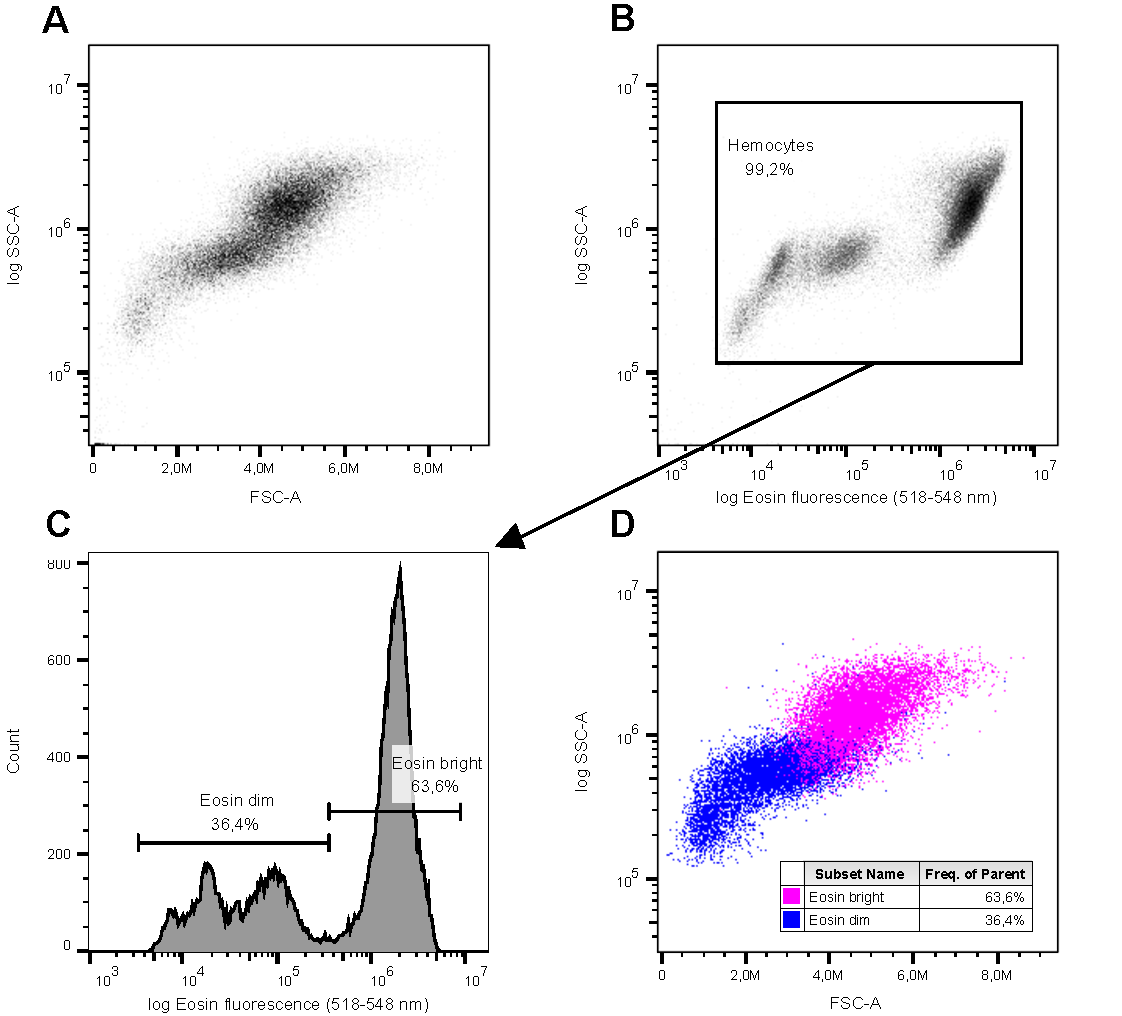
\includegraphics[width=.73\textwidth]{figures/Method development/Eosin exp rastered.pdf}
    \caption{\textbf{Identification eosinophilic granulocytes. A)} Representative light scatter profiles of... \textbf{B)} }
    \label{fig:eosin_exp2}
\end{figure}

[After the eosinophils had sedimented in the \acrshort{mas} buffer (sample M2 in sedimentation dataset) for 2 hours post-withdrawal (1:1), the percentage of eosinophils remaining in suspension were 72/1075 = 6.6976 \%. The 10k ToPro3 Calcein stained plot shows 7.91\%.]
\newpage

In some adult mussels, however, the basophilic and eosinophilic granulocyte subpopulations are partly overlapping with regard to internal complexity, i.e., SSC. Since the BD Accuri C6 Plus isn't equipped with adjustable laser gain settings, these subpopulations could not be separated further instrumentally. Thus, any attempts to gate on these subpopulations based solely on light scattering profiles, would in some mussels introduce considerable uncertainty into their relative proportions. [Find the proportion of mussels where they are not well separated, and report that number instead of saying "some" mussels here.]

End this section by discussing the identity of cluster 1, 2 and 3 in light of availible scientific data, i.e., Le Foll et a. (2010) and Garcia-Garcia et al. (2008). There exists other papers, but they have not verified or at all tested anything and the quality of their flow data is useless. Begin with the following: Le Foll and Colleagues (2010) reached the same conclusion regarding the identity of events populating cluster 3 in Figure \ref{fig:fsc_vs_ssc}. They did however not distinguish between two blast-like basophils and basophillic granulocytes, which led to them to believe that cluster 1 (cluster 3 in LeFoll et al. (2010)) was populated by "basophils" as a whole. Cluster 2 was thought to correspond to hyalinocytes [this requires a meticulous description, since their discussion is so extensive and detailed].

\subsection{Scoring of necrotic haemocytes by flow cytometry}
\subsubsection{Determination of optimal TO-PRO$^{TM}$-3 Iodide staining concentration}
Viable and \ce{MeOH}-killed haemocytes could be separated according to TO-PRO-3 Iodide fluorescence in the whole range of tested concentrations (30 nM - 8 \micro M). As shown in Figure \ref{fig:ToPro3_stain_opt}B, the resolution between ToPro3$^{-}$ and ToPro3$^{+}$ events increased with the TO-PRO$^{TM}$-3 Iodide concentration according to the log-logistic function shown in (\ref{eq:fitted.LL4}), with a marked stagnation > 1.2 \micro M. The model explained almost all the variation in the dataset (Pseudo-R$^{2}$ = 0.99, see table \ref{tb:loglogistic_ToPro3}), and should therefore be a good predictor of the expected resolution between necrotic and viable haemocytes in the tested range of TO-PRO$^{TM}$-3 Iodide.

\begin{equation}
\label{eq:fitted.LL4}
y_{i} = \dfrac{9890700}{1 + (x_i / 0.41655)^{-0.94088}} + \epsilon_i
\end{equation}

The predicted difference in \acrshort{mfi} at 1.2 \micro M was 7.220.000 (arbitrary units), 95\% PI[6.170.000, 8.260.000]. Since the slope of function \ref{eq:fitted.LL4} decreased rapidly for x > 0.6, the predicted difference in MFI at x = 1.2 \micro M was contained within the prediction intervals for the rest of the function's range. Furthermore, the MFI of the ToPro3$^{-}$ populations increased abruptly at concentrations $\geq$ 2 \micro M (see Table \ref{tb:ToPro3_stainopt}), indicating a potential cytotoxic effect of either TO-PRO$^{TM}$-3 Iodide or the \acrshort{dmso} solvent at high concentrations.

\begin{figure}[h]
    \centering
    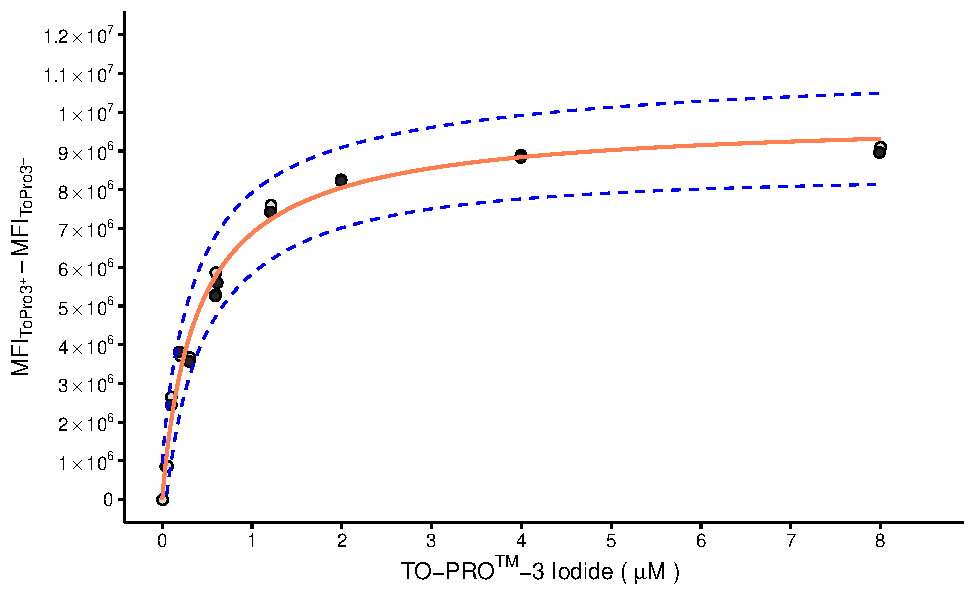
\includegraphics[width=1.0\textwidth]{figures/Method development/ToPro3 LL4.pdf}
    \caption{\textbf{Experimental determination of the optimal TO-PRO$^{TM}$-3 Iodide concentration for a dye exclusion test of membrane integrity}. 10 aliquots of pooled methanol-killed (70\% \ce{MeOH}, 30 min) and viable haemocytes (1:1) were stained with different concentrations of TO-PRO$^{TM}$-3 Iodide (30 nM - 8 \micro M). 640 nm-exited fluorescence from \acrshort{dsdna}-bound TO-PRO$^{TM}$-3 Iodide were collected on the FL4 detector (675/25 nm) of the BD Accuri C6 Plus flow cytometer, recording 10.000 events from each sample after 15 and 30 minute incubation. \textbf{A)} ToPro3$^{-}$ and ToPro3$^{+}$ events were gated on log scale for each sample, \textbf{B)} and their difference in mean fluorescent intensity (MFI) after 15 (\protect\lysegraacircle) and 30 minutes (\protect\darkgraycircle) of incubation were plotted against the concentration of TO-PRO$^{TM}$-3 Iodide. Red line: fitted log-logistic regression model; blue dashed lines: prediction intervals.}
    \label{fig:ToPro3_stain_opt}
\end{figure}

Taken together, these results suggested that the potential gain from increasing the staining concentration above 1.2 \micro M was limited, and not completely free of risk. The resolution between viable and necrotic haemocytes was for all practical purposes sufficient the range of 300 nm - 1.2 \micro M, but the resolution at 1.2 \micro M would simplify gating on a logarithmic scale. 1.2 \micro M TO-PRO$^{TM}$-3 Iodide was therefore preferred for scoring necrotic haemocytes by flow cytometry, together with 50 nM Calcein AM.

The results were also unambiguous regarding the incubation period. According to Figure \ref{fig:ToPro3_stain_opt}B, the resolution between viable and necrotic cells did not increase after the initial 15 minute incubation period. The MFI of necrotic haemocytes did increase somewhat in the extended incubation period, but the resolution remained unchanged due to a concurrent proportional increase among the viable haemocytes (see table \ref{tb:ToPro3_stainopt}, Appendix B). Extending the incubation period beyond 15 minutes would therefore be of little use.

\subsubsection{Method validation}
Simple linear regression was used to examine the correlation between results obtained by epifluorescent microscopy and the flow cytometric gating strategy presented in section \ref{subsubsection: gating validation}. It was found that the established quadrant gating strategy significantly predicted the the percentage of ToPro3$^{+}$ haemocytes (\%) in samples scored by epifluorescent microscopy ($\beta$ = 0.98818, t(8) = 32.8, p<.001). The data is presented in Figure \ref{fig:method_val_1}, together with the fitted linear regression model (R$^{2}$ = 0.99, F(1, 8) = 1059, p<.001).

\begin{figure}[h]
    \centering
    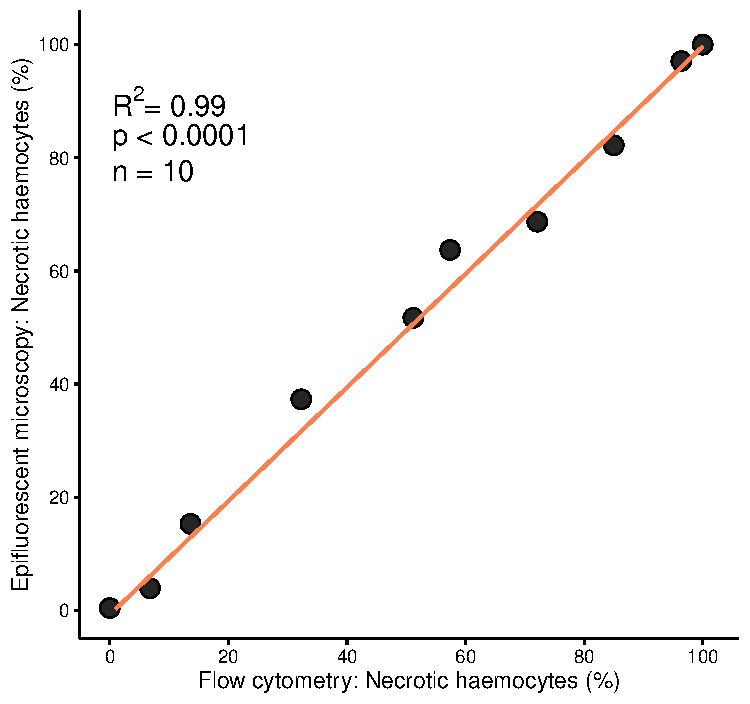
\includegraphics[width=.65\textwidth]{figures/Method development/FCM FM lin reg.pdf}
    \caption{\textbf{Correlation between necrotic haemocyte percentages scored by flow cytometry and epifluorescent microscopy.} 10 samples of freshly withdrawn haemocytes (\acrshort{acb}, 1:1) were mixed with methanol-killed haemocytes in semi-random proportions (0-100\%), stained with Calcein AM (50 nM) and TO-PRO$^{TM}$-3 Iodide (1.2 \micro M) and the percentage of necrotic haemocytes (\%) were scored by both flow cytometry and epifluorescent microscopy. Each datapoint represents one scored sample. Red line: fitted linear regression model.}
    \label{fig:method_val_1}
\end{figure}



\newpage
\section{Hybrid FCM/Microscopy MN Cytome Assay: Results}
\subsection{MN and other nuclear anomalies}
\subsection{Haemocyte viability: membrane integrity}
\subsection{Apoptosis assay}
\subsection{Haemocyte differential counts and concentration}

